% https://opensource.com/resources/what-docker
Docker is an open\hyp{}source tool designed to simplify the creation, deployment, and running process of applications through the usage of containers. Containers allow the packaging of an application with all of the parts it needs, such as libraries and other dependencies. The application will run on any Linux machine regardless of any customized settings of that machine, because of the isolation of these containers. \cite{opensource_what_is_docker}

% https://opensource.com/resources/what-docker
Often the comparison is made with a \ac{vm}. But unlike a \acs{vm}, Docker does not need virtualization of a whole operating system. The applications run by Docker use the same Linux kernel as the host system. Therefore, compared to a \acs{vm}, it has a significant reduction in size and a boost in performance. \cite{opensource_what_is_docker}

% https://davidsoff.nl/presentation/docker-101/#1
\begin{figure}[!h]
    \centering
    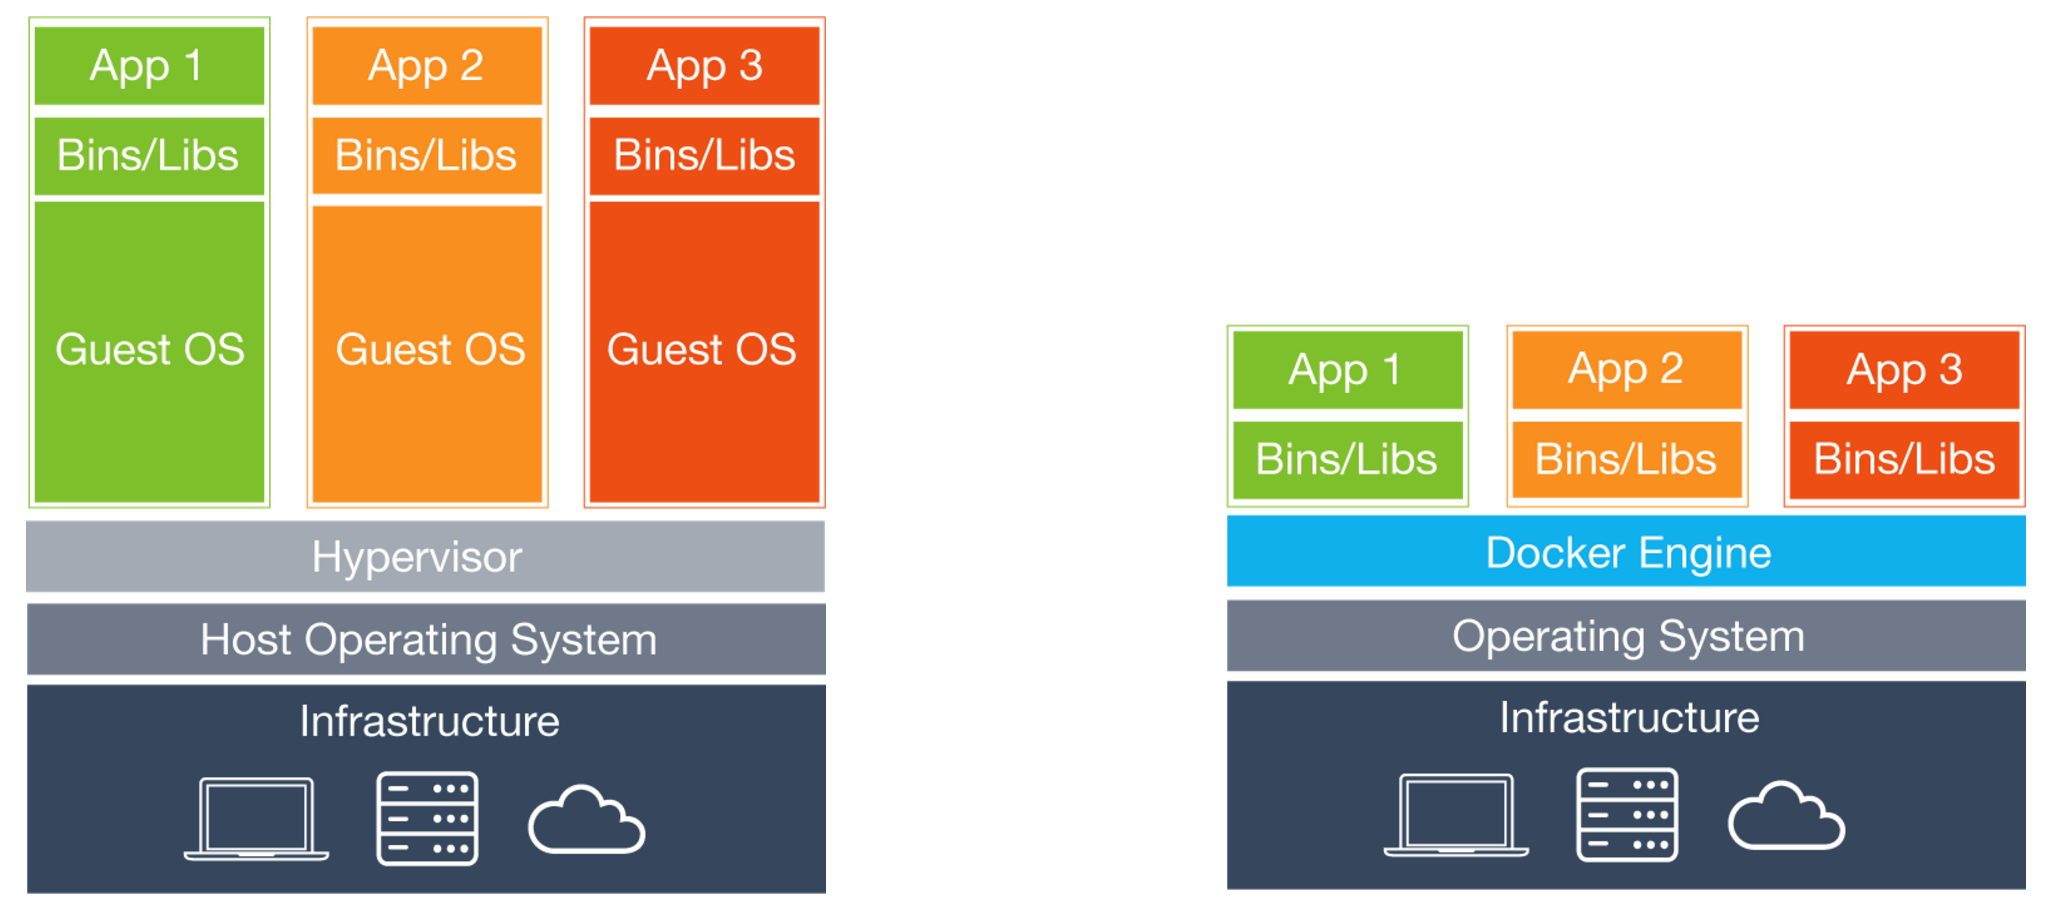
\includegraphics[width=0.8\linewidth]{images/vm_vs_container.png}
    \caption{Virtual Machine versus Docker container}
    \label{fig:vm_vs_container}
\end{figure}

% https://docs.docker.com/get-started/overview/
Running Docker containers requires images. An image is a read\hyp{}only template with commands for creating a container. These images can be obtained by two methods: creating your own or pulling from a registry. Pulling an image from a registry is the equivalent of downloading from the internet, these images are premade. Building your image requires a Dockerfile, in this file a set of Docker commands are defined that define the image. A container is a runnable instance of an image. This container can be started, stopped, moved, or deleted. After modifying the container, it can be saved back to an image for later use. The image can then be pushed back to the registry. \cite{docker_get_started_overview}

This project mainly uses Docker for an isolation option lighter than a virtual machine, its consistency, and scalability. However, the increased freedom is also a bonus. Knowing there is always a stable backup no matter which software or packages you experiment with.